\documentclass[10pt,sans-serif]{beamer}
\usepackage{amsmath}
\usepackage{concrete}
\usetheme{Madrid}
\usecolortheme{rose}
\usefonttheme{structuresmallcapsserif}
\usepackage{bookman}

\title[TDA]{Discrete Morse Theory and Applications in TDA}

\author[Sush]{Sushovan ``\textcolor{magenta}{Sush}'' MAJHI} \date[Tulane
  University '19]{Wenk's Team Meeting \\ Tulane University, 2019}

\begin{document}
\frame{\titlepage}


\begin{frame}{}
  I am a \textcolor{magenta}{fifth year} Math PhD student at Tulane University.
  \\
  \vspace{50pt}
  \textbf{Thesis Advisor:}\\
  \textcolor{blue}{Carola Wenk}, Computer Science, Tulane University\\

  \vspace{50pt} \textbf{My Collaborators:}\\ \textcolor{blue}{Rafal
    Komendarczyk}, Mathematics, Tulane University \\ \textcolor{blue}{Brittany
    Terese Fasy}, Computer Science, Montana State University
  \\ \textcolor{blue}{Yusu Wang}, Computer Science, Ohio State University
\end{frame}

\begin{frame}{Topological Data Analysis (\textcolor{yellow}{TDA})}
  \begin{block}{What is TDA?}
    TDA is a subfield of applied mathematics. Topological tools and techniques
    are used to \textcolor{blue}{Simplify}, \textcolor{magenta}{Analyze} and
    \textcolor{red}{Visualize} data.
  \end{block}

  \pause

  \begin{block}{What tools are used?}
    Simplicial Homology, Simple Homotopy Theory, Persistent Homology, Metric
    Geometry, Morse Theory etc.
  \end{block}
  
\end{frame}

\font\tenipa=tipa12
\def\schwa{{\tenipa\char64}}

\begin{frame}{}
  \begin{block}{}
    {\huge data } \textcolor{gray}{(dictionary.cambridge.org)}\\
    
    \textcolor{gray}{noun [U, sing/pl verb]}$\bullet$ \textcolor{red}{US}
    \textcolor{magenta}{/de\textrm{I}.t\schwa/} \\
    
    information, especially facts or numbers, collected to be examined and
    considered and used to help decision-making, or information in an electronic
    form that can be stored and used by a computer.
  \end{block}

  \pause
  
  \begin{block}{}
    Data is an incomplete and \textcolor{magenta}{discrete} projection (sample)
    of a rather \textcolor{magenta}{continuous} object of interest.
  \end{block}
\end{frame}

\begin{frame}{Universal Truth about Data}
  \begin{enumerate}
  \item full of noise/error/outliers
  \item incomplete
  \item high-dimensional
  \end{enumerate}

  \pause

  \vspace{12pt}
  \textbf{Still we trust our data!}
  \begin{figure}
    \centering
    
\includegraphics[scale=0.35]{trust-the-data}
    \caption{Joke from \textcolor{gray}{bigdata-madesimple.com}}
  \end{figure}
\end{frame}

\begin{frame}{Data Analysis}

  \begin{block}{}
    Extract info about the continuous object being sampled.
  \end{block}

  \pause
  
  \begin{block}{}
    \begin{enumerate}
    \item Statistical Data Analysis (using hyperplanes, hypersurfaces, PDEs
      etc.)
    \item Smooth Interpolation
    \item Fractal Interpolation
    \end{enumerate}
  \end{block}
\end{frame}


\begin{frame}{Why TDA?}
  \begin{block}{}
    Some data are very geometric in nature e.g. medical images, 3D printing.
  \end{block}
  \begin{figure}
    \centering
    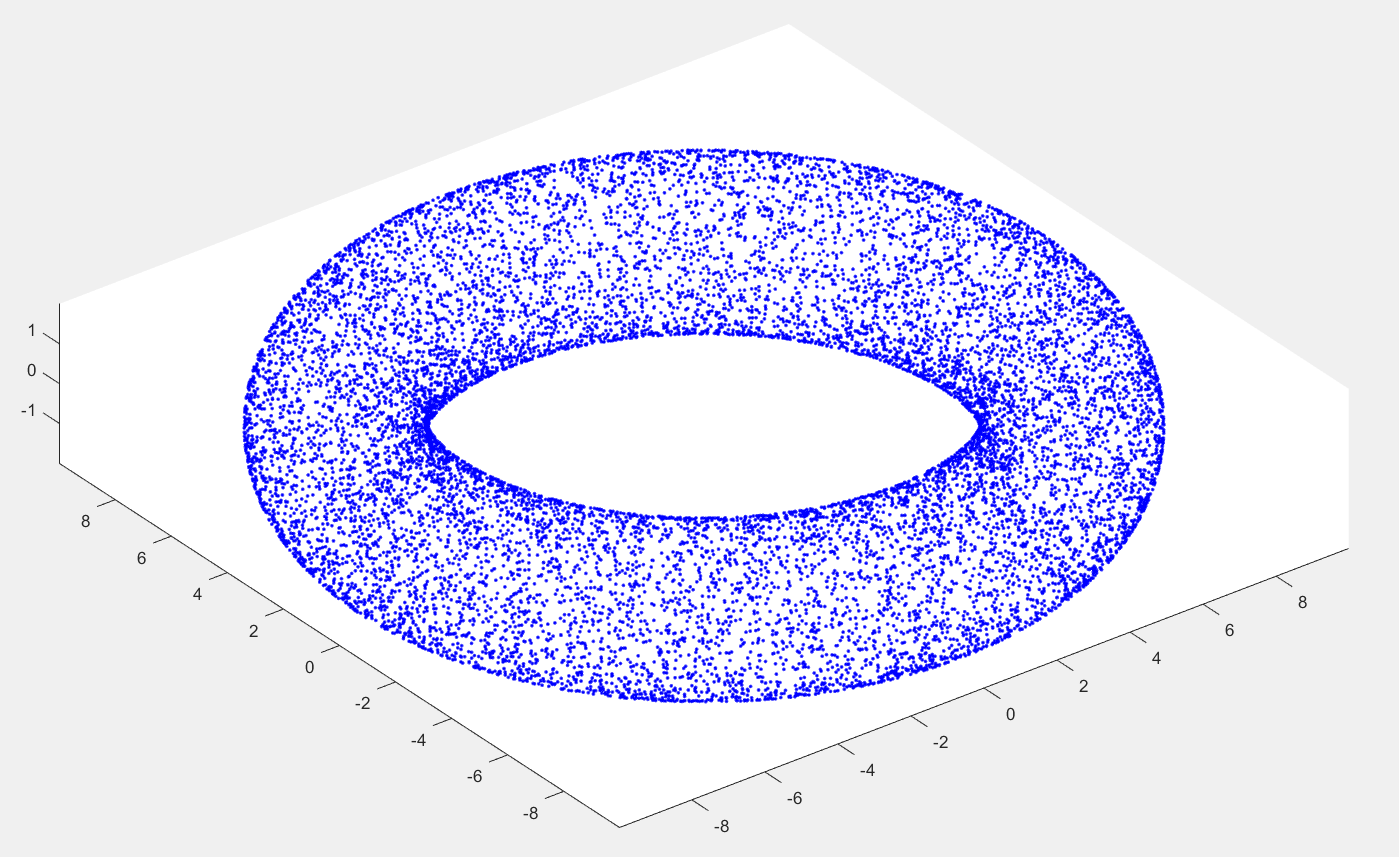
\includegraphics[scale=0.3]{torus}
    \caption{A sample from an embedded Torus 
      (\textcolor{gray}{Matlab\textsuperscript\textregistered})}
  \end{figure}
\end{frame}

\begin{frame}{Why TDA?}
  \begin{figure}
    \centering
    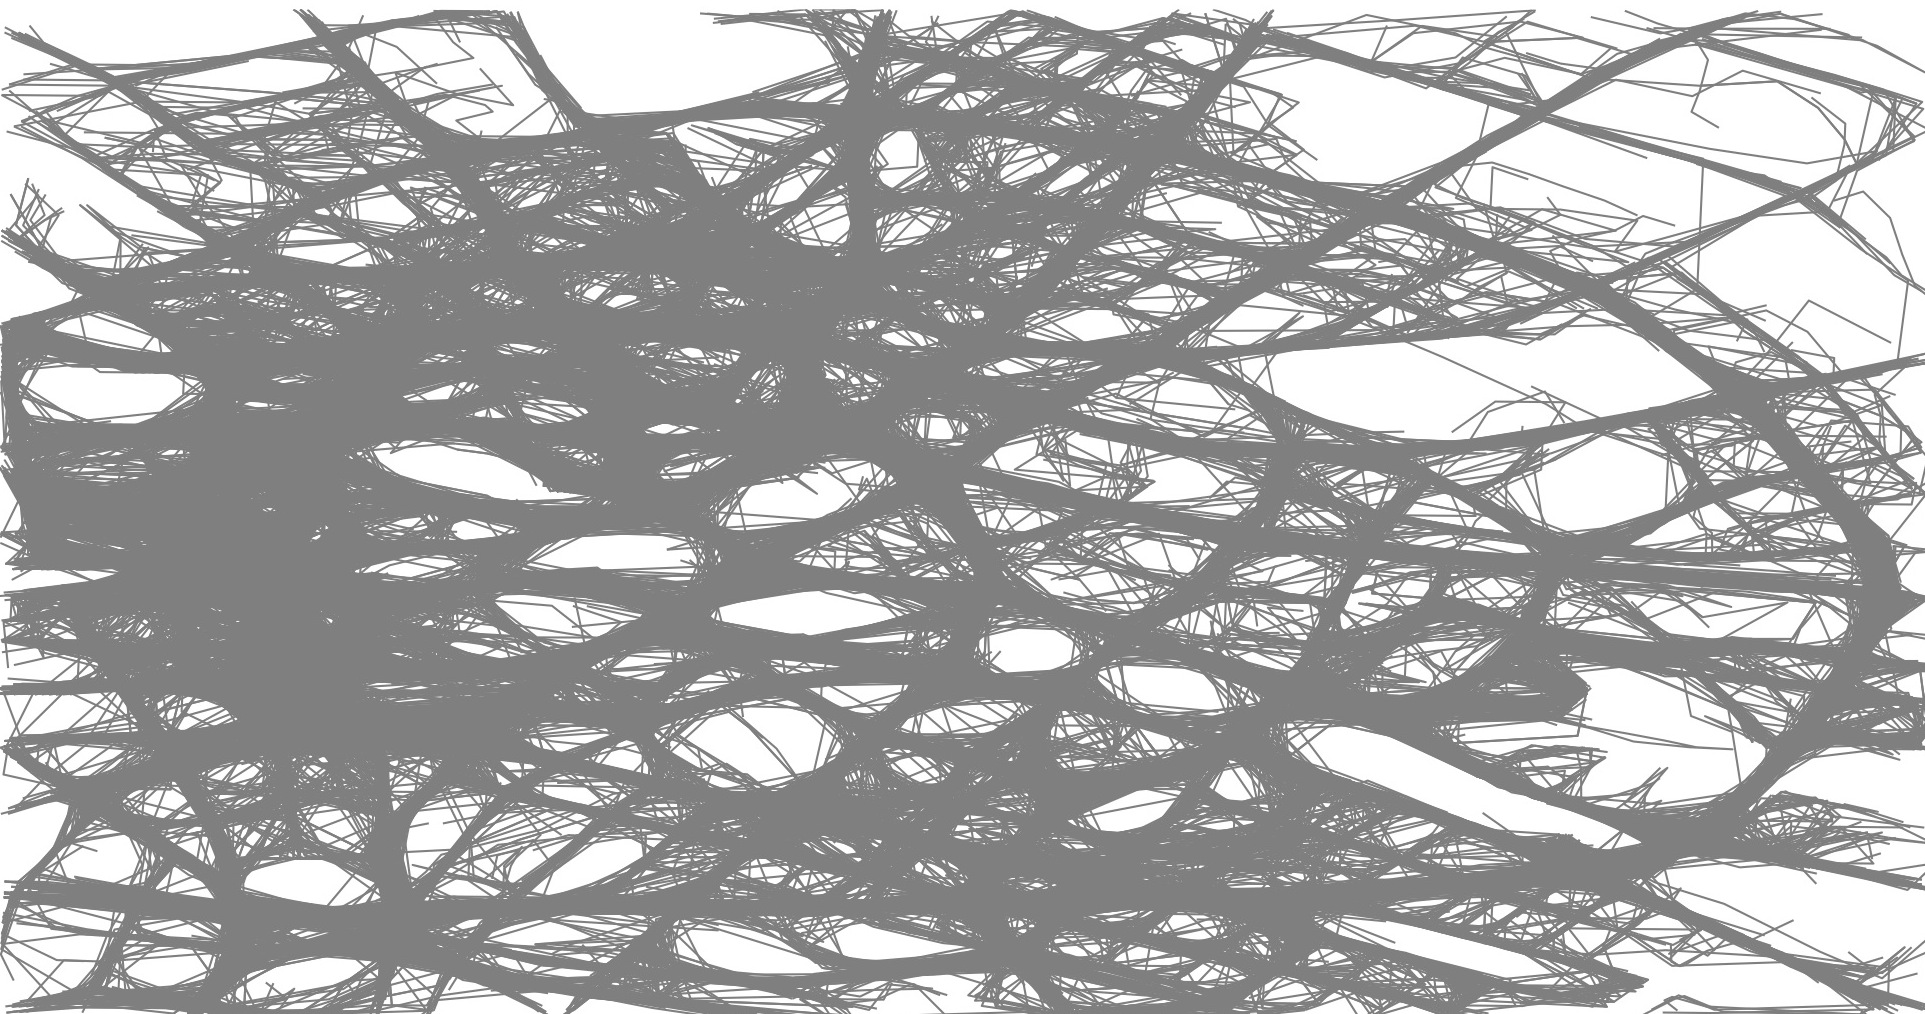
\includegraphics[scale=0.3]{Berlin}
    \caption{GPS traces of Berlin, Germany
      (\textcolor{gray}{www.mapconstruction.org})}
  \end{figure}
\end{frame}

\begin{frame}{Why TDA?}
  \begin{figure}
    \centering
    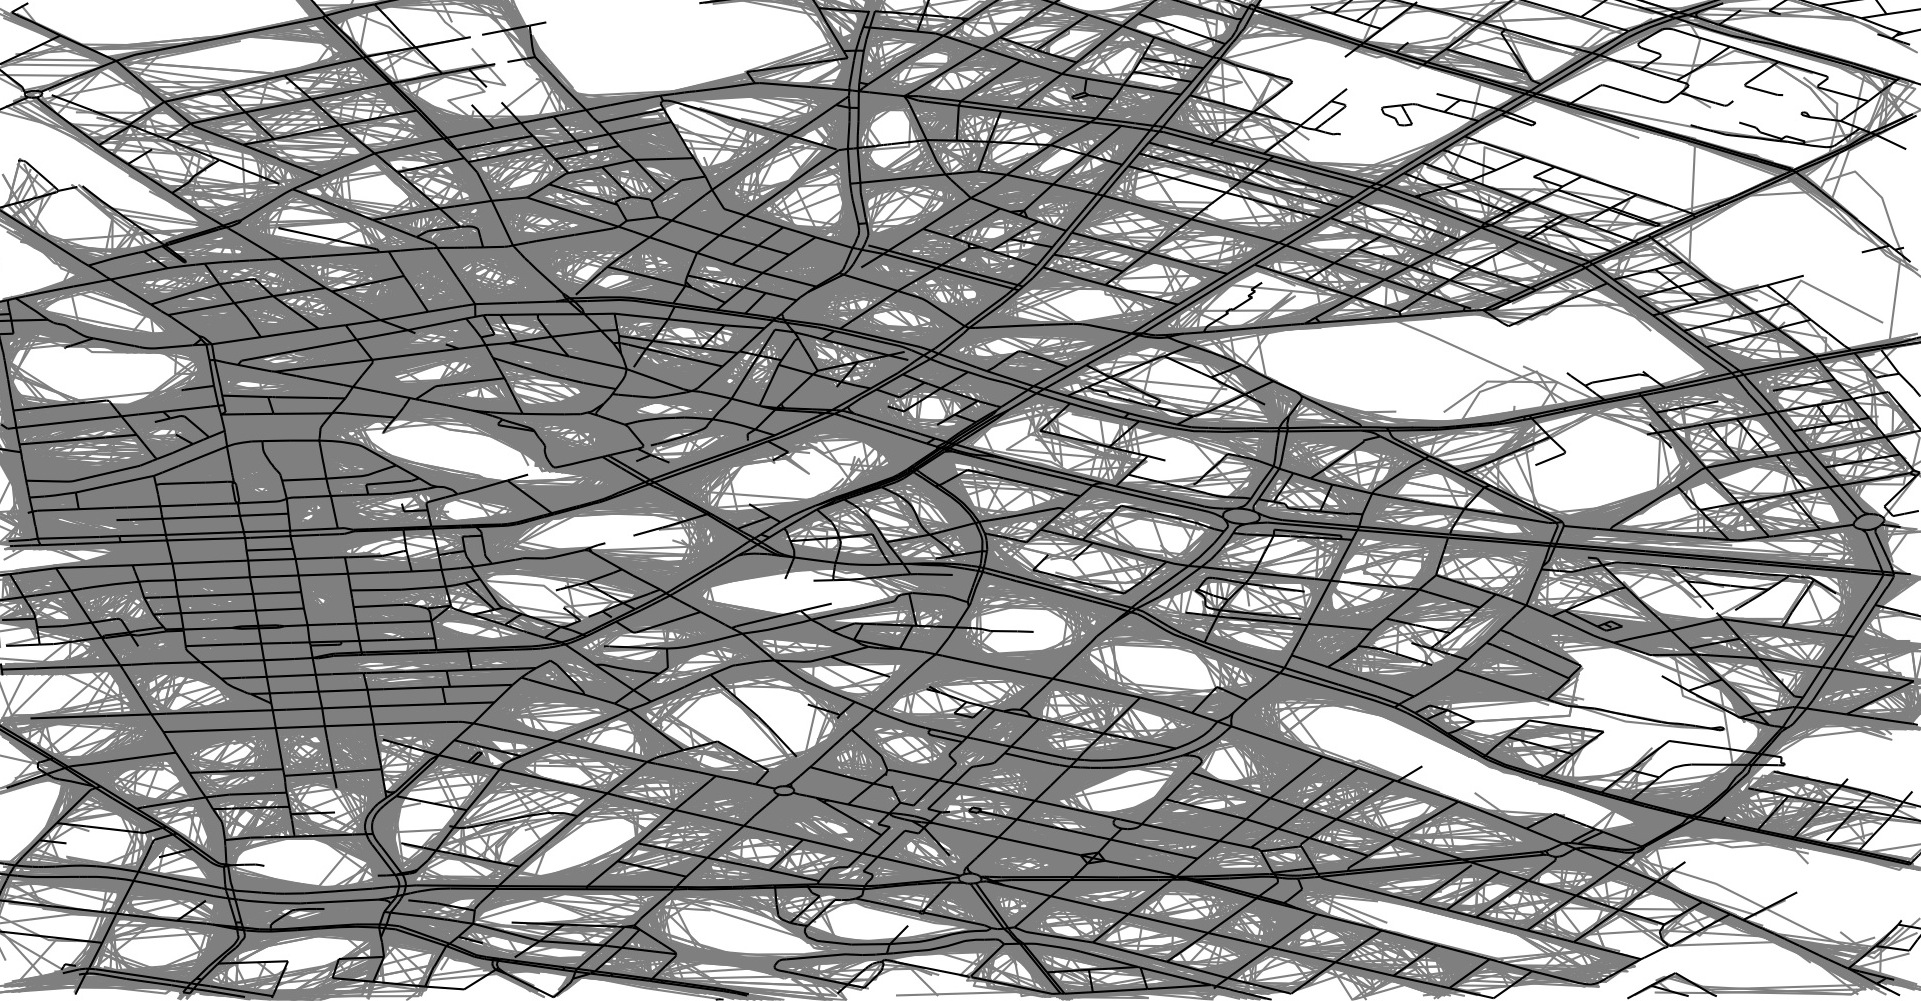
\includegraphics[scale=0.3]{Berlin_Recon}
    \caption{A possible reconstruction of road-network
      (\textcolor{gray}{www.mapconstruction.org})}
  \end{figure}
\end{frame}


\begin{frame}{Problem of Map Reconstruction}
  \begin{block}{Applied math is also Challenging!}
    A real-world problem does not directly inform us about the math behind it.
  \end{block}

  \pause
    \begin{block}{Our Problem}
    GPS traces $\to$ road-network
  \end{block}

  \pause
  
  \begin{block}{Expectations}
    \begin{enumerate}
    \item The output is homotopy equivalent to the actual road-network
      i.e. \textcolor{magenta}{same homology, homotopy groups}.
    \item output has a very small Hausdorff distance to the ground truth i.e.
      \textcolor{magenta}{close geometric features as well}.
    \end{enumerate}
  \end{block}
\end{frame}

\begin{frame}{Our First Approach}
  \begin{block}{Tools Used}
    \textcolor{magenta}{Metric Geometry} (geodesic space, Gromov distortion,
    convexity radius) \\
    \vspace{20pt} \textcolor{magenta}{Algebraic Topology} (Cech and Vietoris-Rips
    complexes, Simplicial Homology, Simplicial Shadow).
  \end{block}

  \pause
  
  \begin{theorem}[\textcolor{gray}{submitted to SOCG'19}]
    Let $X$ be a compact subset of~$\mathbb{R}^N$ with a positive convexity
    radius $\rho$ and finite distortion $\delta$. And, let $S \subseteq
    \mathbb{R}^n$ such that
    $d_H(S,X)<\epsilon<\frac{\rho}{4\delta(2\delta+1)}$. Then, for any
    non-negative integer $k$, $H_k(X)$ is isomorphic to the image of the
    homomorphism induced by the following simplicial inclusion~map
    $$j:\mathcal{C}_\epsilon(S)\to\mathcal{C}_{(4\delta+1)\epsilon}(S).$$
  \end{theorem}
\end{frame}


\begin{frame}{The Shortcomings}  
  \begin{figure}
    \centering
    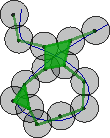
\includegraphics[scale=1.8]{graph-recon}
    \caption{Reconstruction of a planar graph}
  \end{figure}

  \pause

  \begin{block}{}
    \begin{enumerate}
    \item the output (green) does not look like a graph
    \item the method does not like outliers
    \end{enumerate}
  \end{block}
\end{frame}

\begin{frame}{Classical Morse Theory}
  \begin{block}{Motivation}
    A reasonably "good'' smooth function reveals the
    \textcolor{blue}{Combinatorial Description} of a smooth manifold.
  \end{block}
\end{frame}


\begin{frame}{Classical Morse Theory}
  Let $M^n$ be a smooth manifold and $f:M\to\mathbb R$ be a smooth function. 
  
  \begin{block}{Critical Point}
    A point $p\in M$ is called a \textcolor{blue}{critical point} of $f$ if
    $Df=0$.
    
    \pause
    \vspace{10pt}
    
    A critical point $p$ is \textcolor{magenta}{non-degenerate} if $Hess(f)$ is
    non-singular. \\
    The number of -ve eigen values if called the \textcolor{red}{index} of $p$.
  \end{block}
  
  
  \pause
  
  \begin{figure}
    \centering
    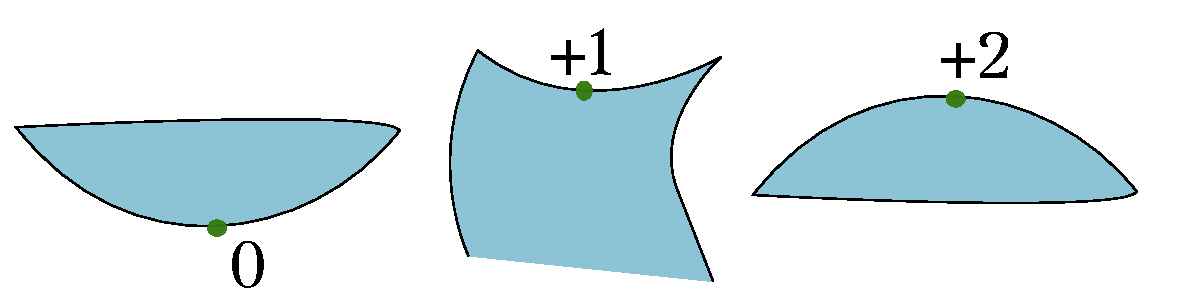
\includegraphics[scale=0.5]{critical}
    \caption{critical points with index}
  \end{figure}

\end{frame}

\begin{frame}{Classical Morse Theory}  
  \begin{block}{Morse Function}
    A smooth function $f:M^n\to\mathbb R$ is called a \textcolor{blue}{Morse
      function} if all its critical points are non-degenerate.  \\ \pause

    $p$ has index \textcolor{magenta}{0}. $w$ has index
    \textcolor{magenta}{+2}. Others have index \textcolor{magenta}{+1}.

  \end{block}
  
  
  \begin{figure}
    \centering
    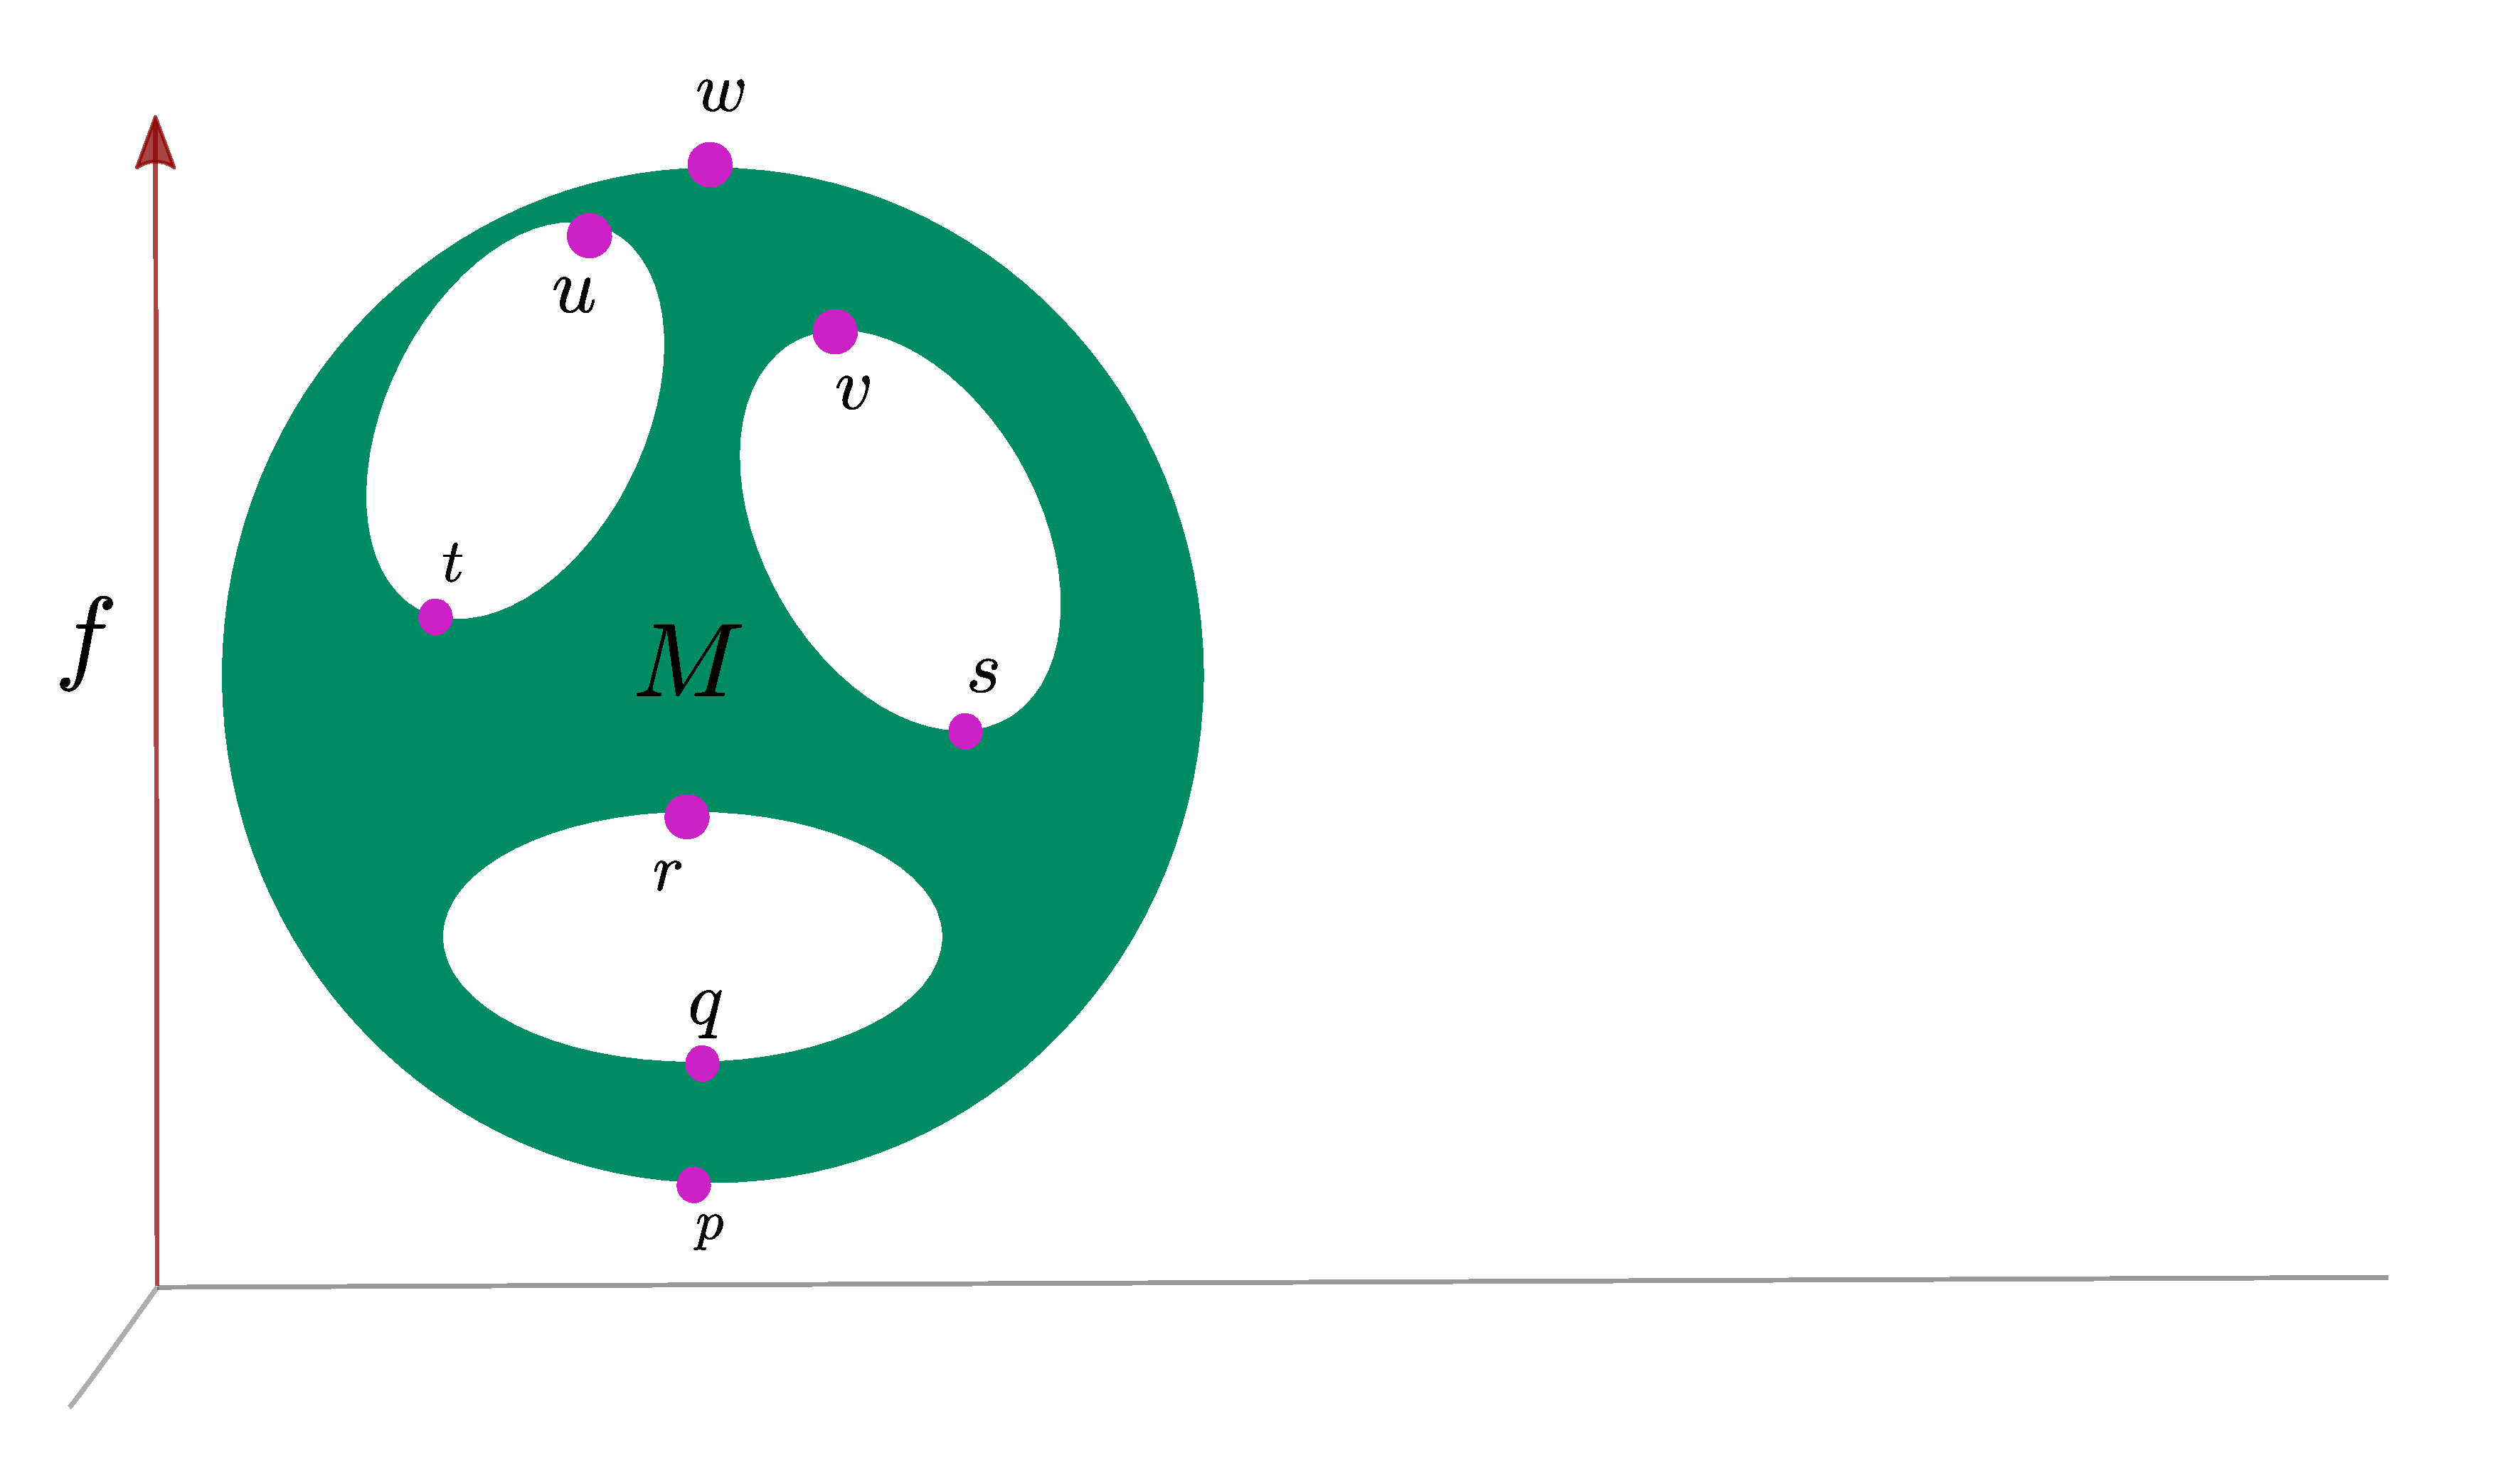
\includegraphics[scale=0.15]{0}
    \caption{Morse Function}
  \end{figure}

\end{frame}


\begin{frame}{Classical Morse Theory}
  \begin{figure}
    \centering
    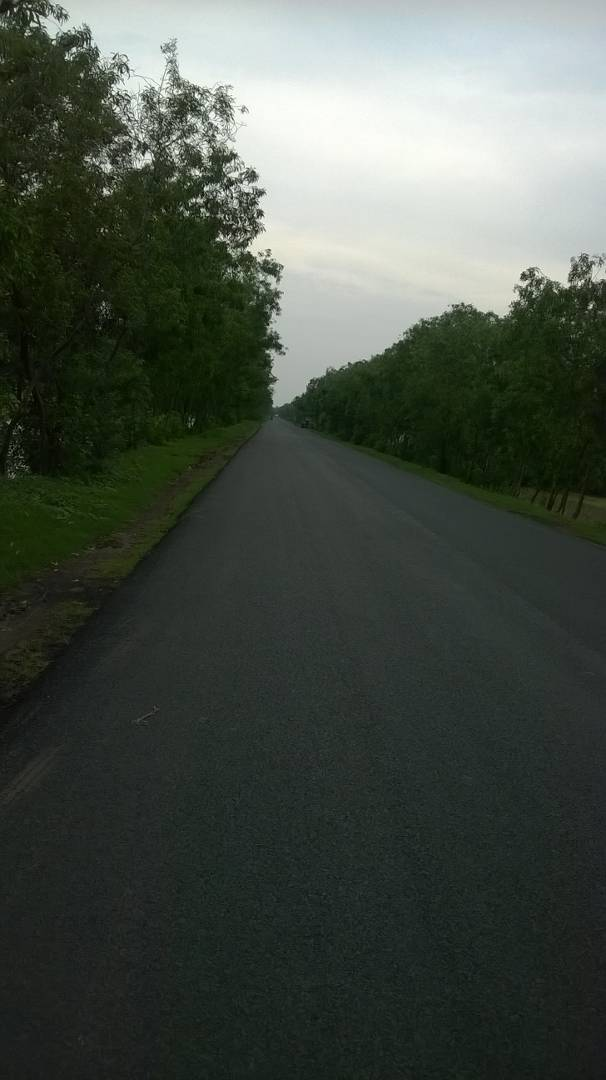
\includegraphics[scale=0.2]{1}
    \caption{Sub-level Set}
  \end{figure}
\end{frame}

\begin{frame}{Classical Morse Theory}  
  \begin{figure}
    \centering
    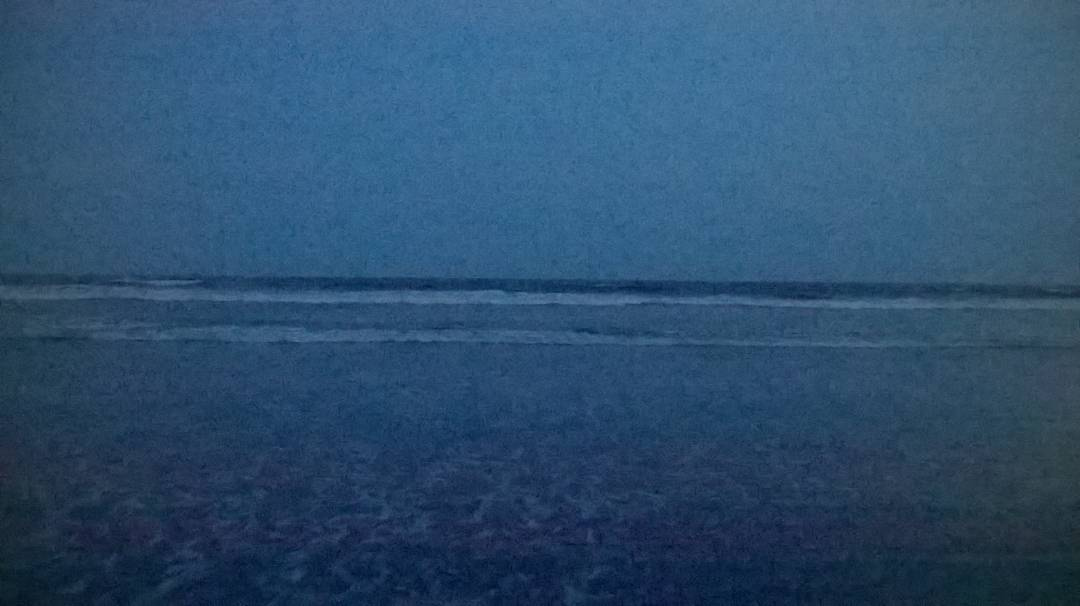
\includegraphics[scale=0.2]{2}
    \caption{Sub-level Set}
  \end{figure}
\end{frame}

\begin{frame}{Classical Morse Theory}
  \begin{figure}
    \centering
    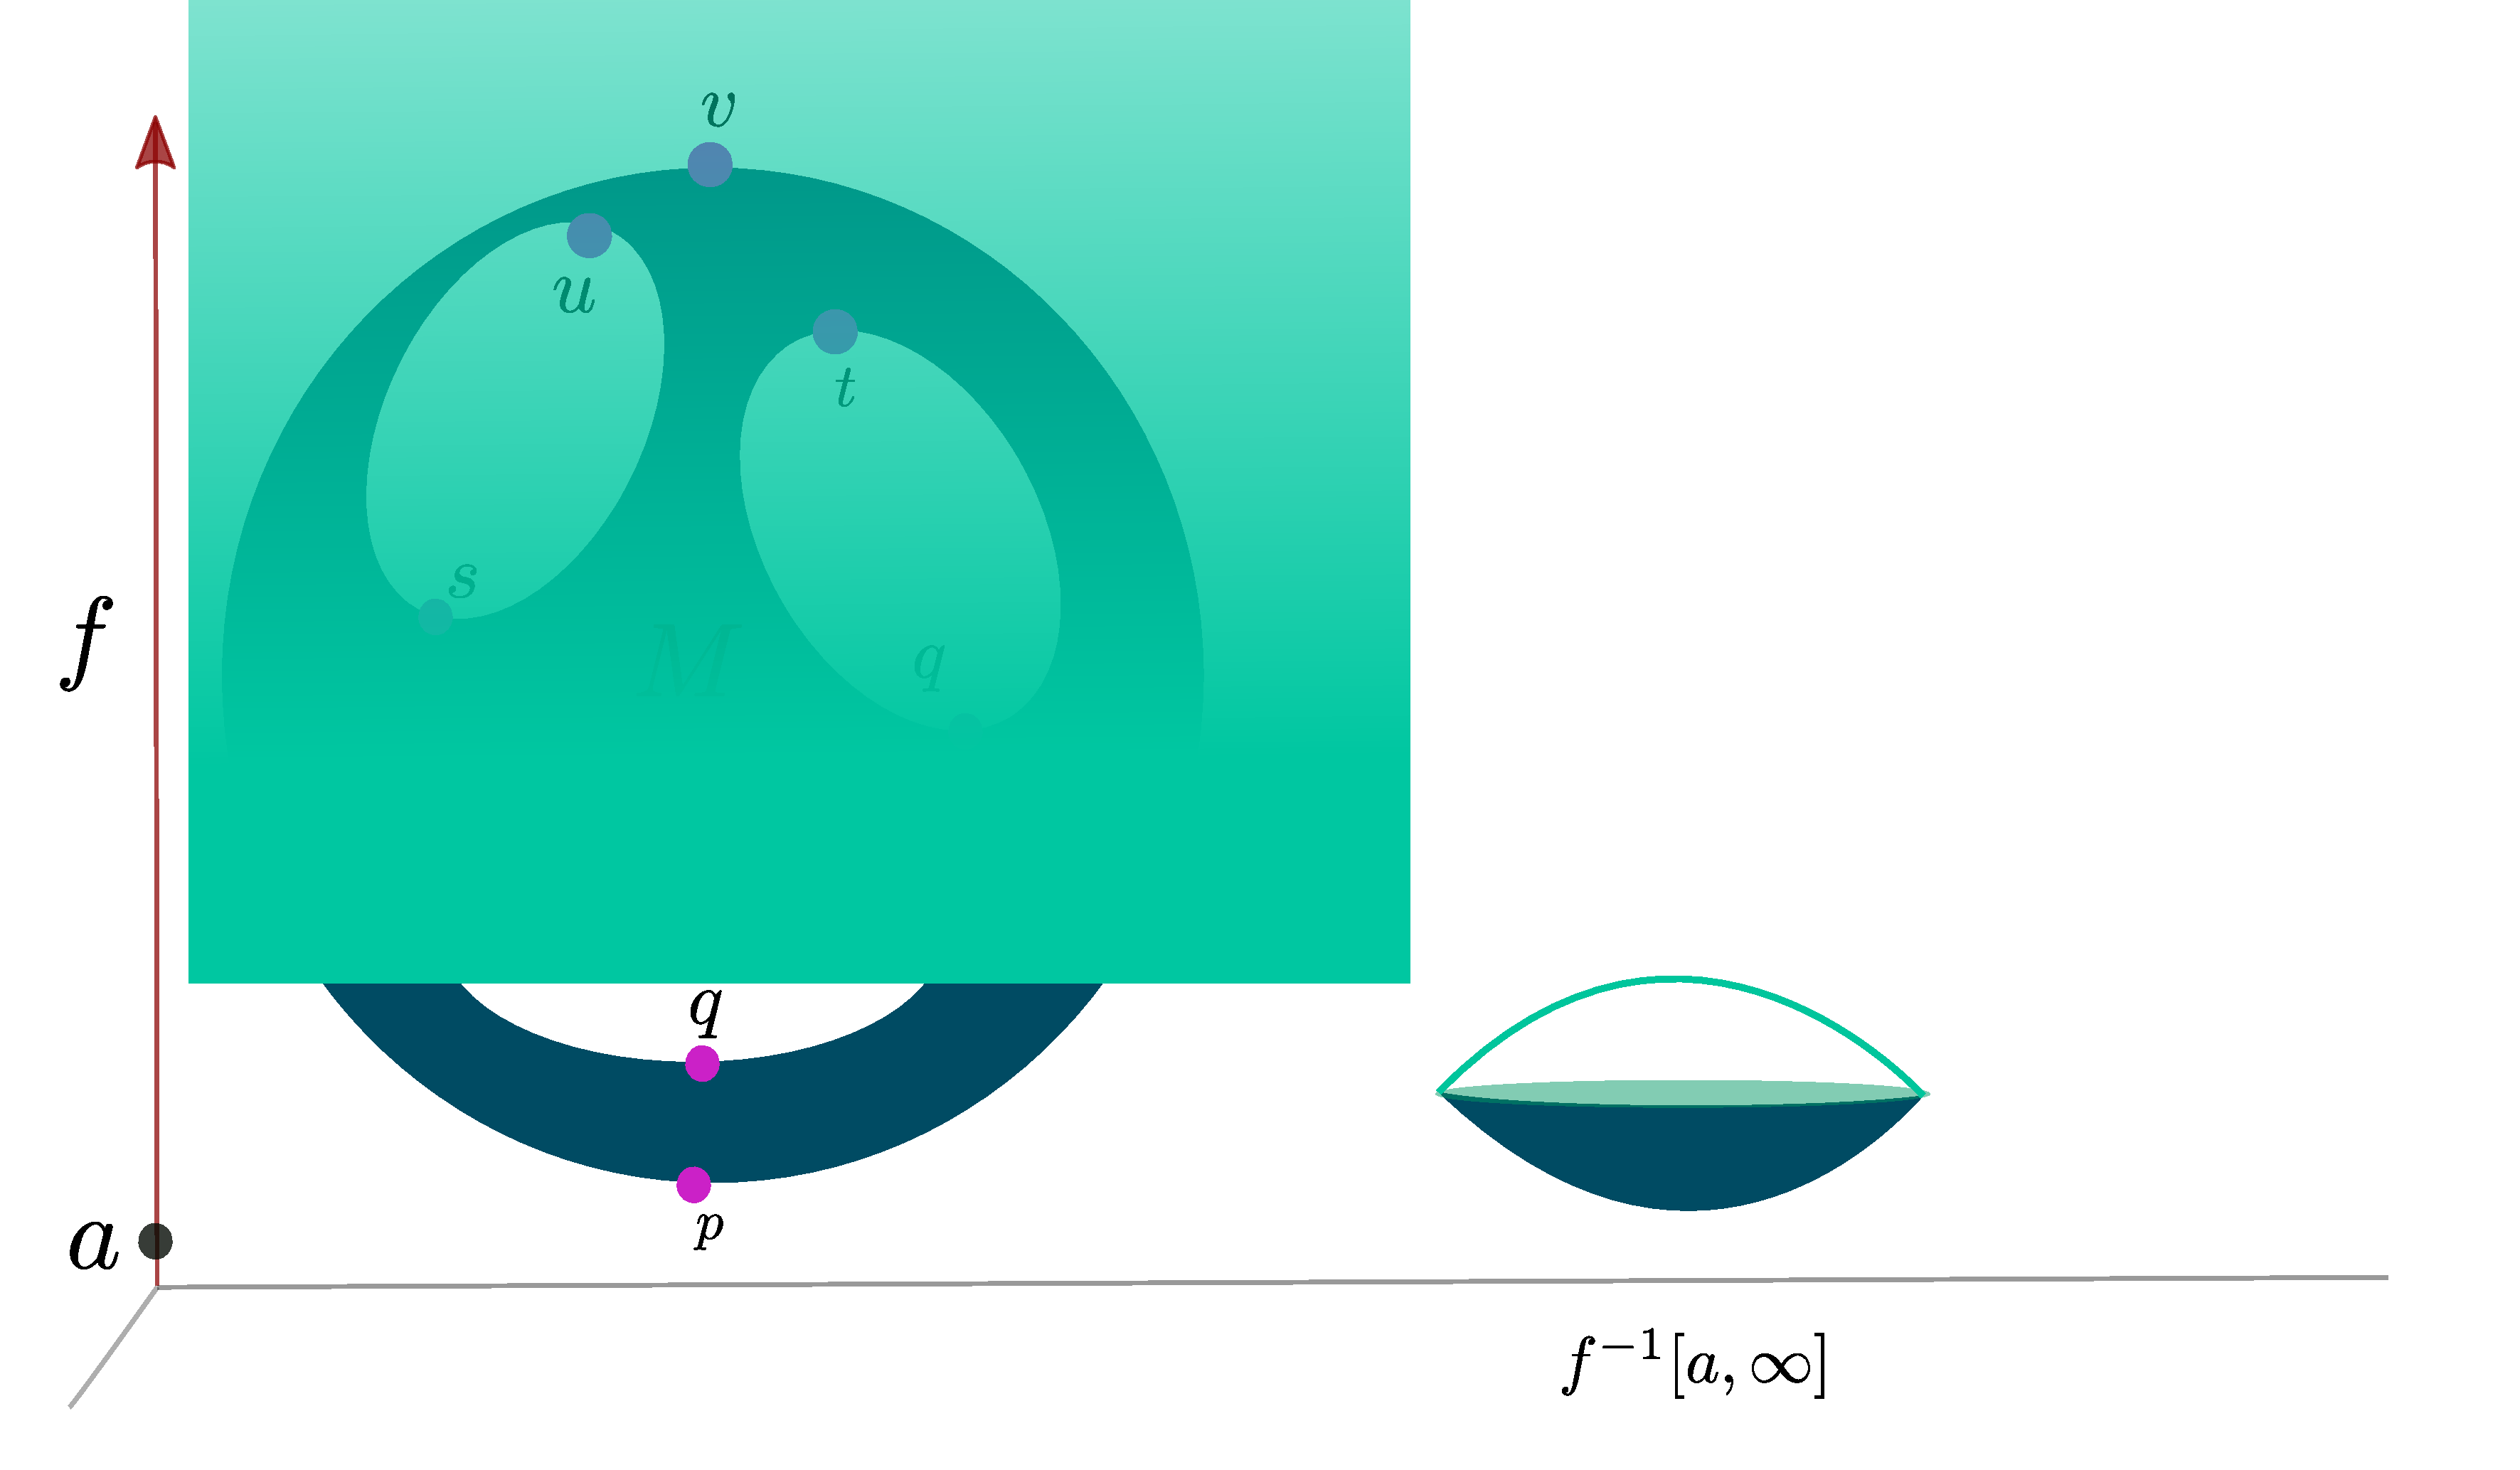
\includegraphics[scale=0.2]{3}
    \caption{Sub-level Set}
  \end{figure}
\end{frame}

\begin{frame}{Classical Morse Theory}
  \begin{figure}
    \centering
    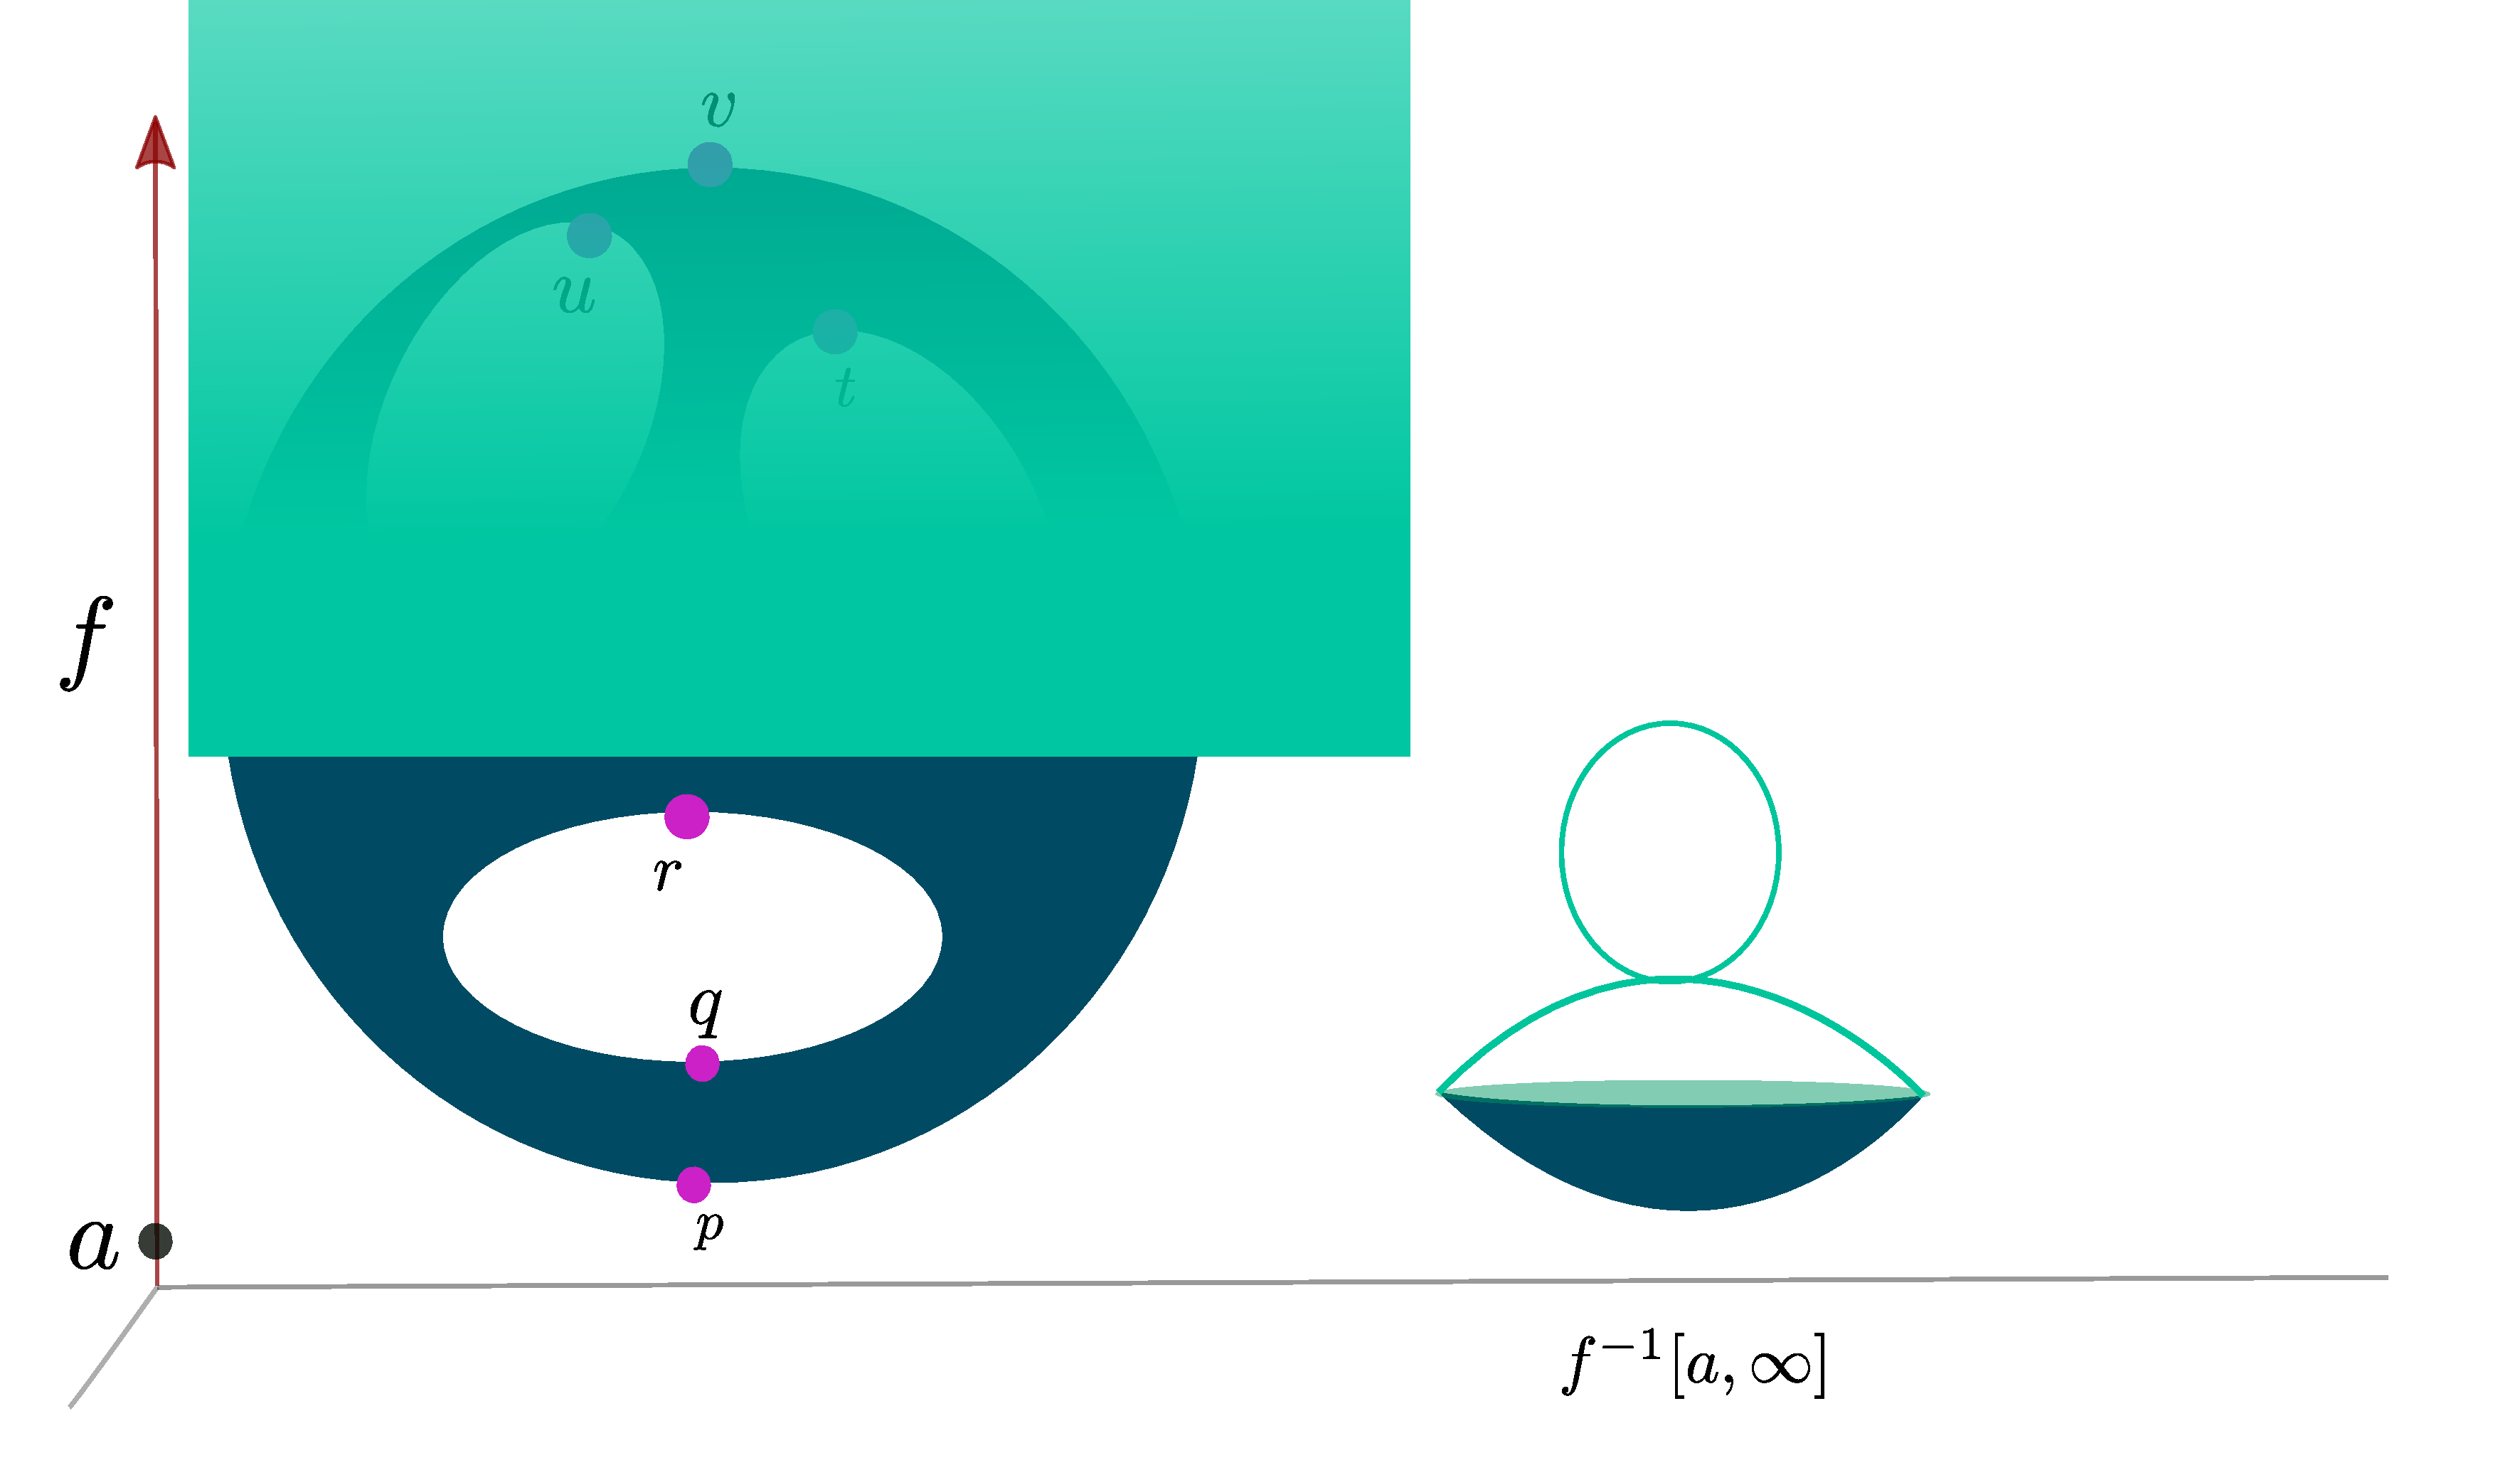
\includegraphics[scale=0.2]{4}
    \caption{Sub-level Set}
  \end{figure}
\end{frame}

\begin{frame}{Classical Morse Theory}
  \begin{figure}
    \centering
    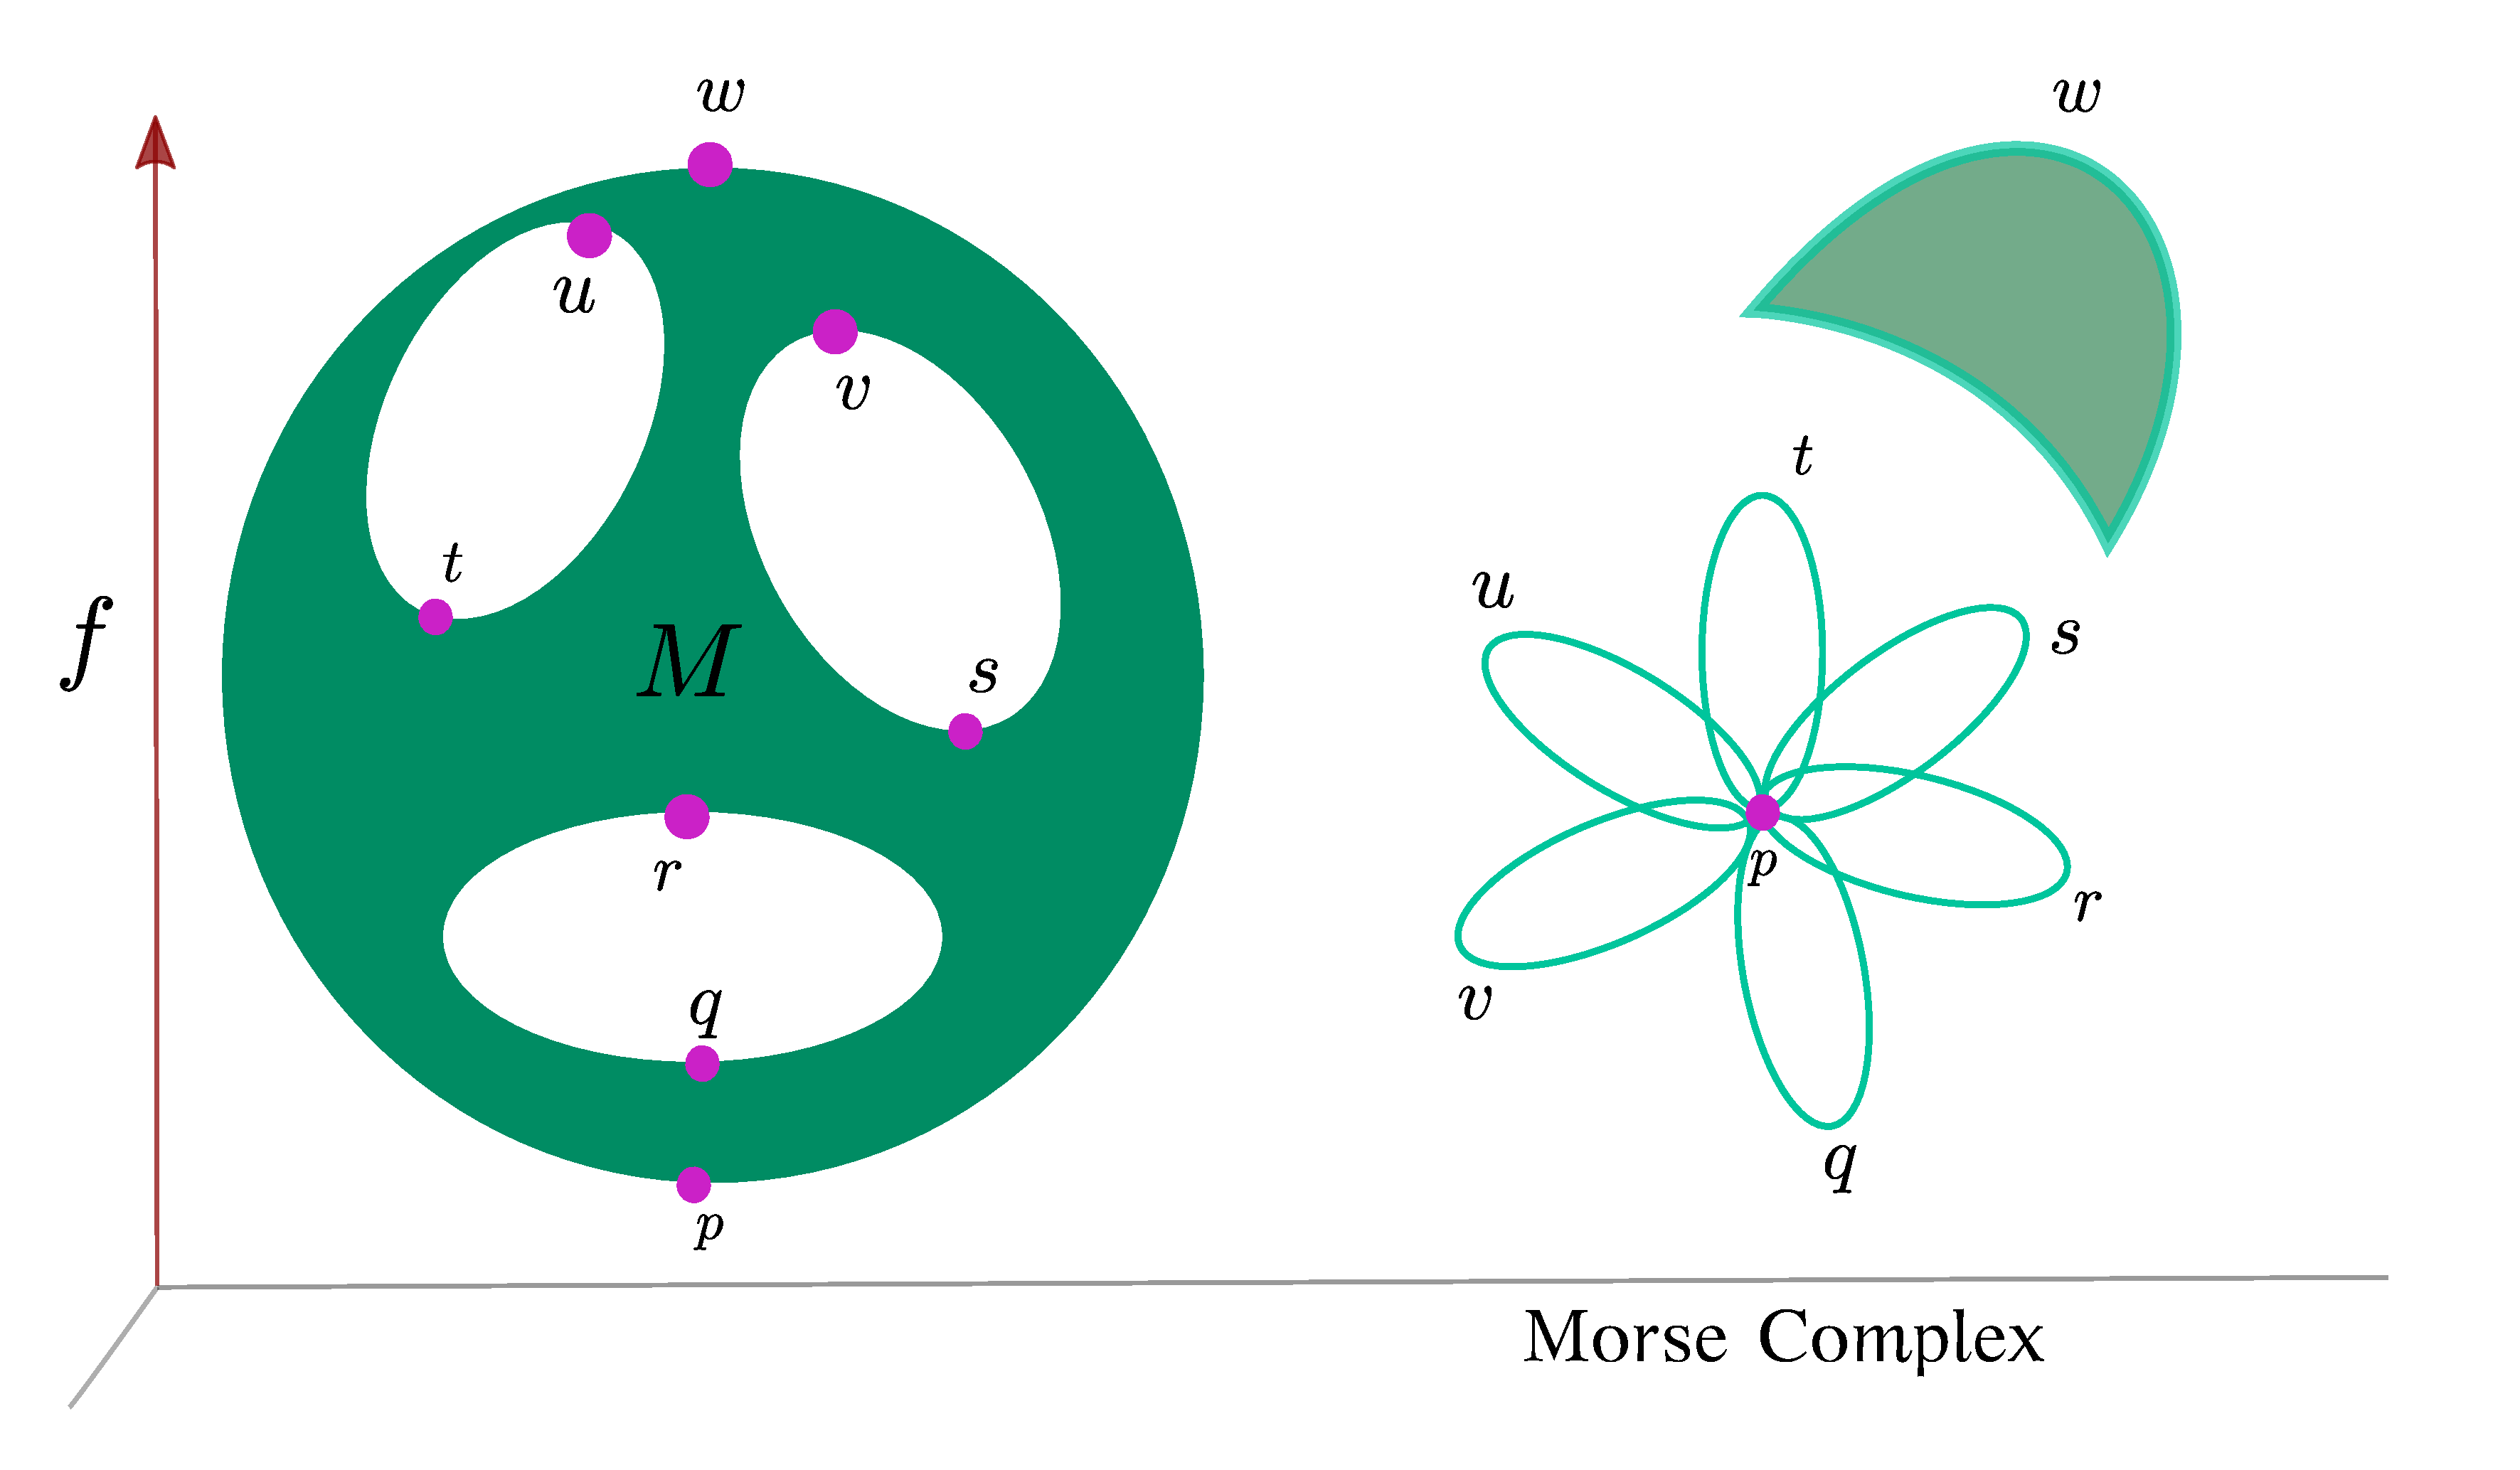
\includegraphics[scale=0.2]{5}
    \caption{Morse Complex}
  \end{figure}
\end{frame}

\begin{frame}{Classical Morse Theory}
  \begin{block}{Morse Theorem}
    If $f$ is Morse on $M$, then $M$ is \emph{homotopy equivalent} to a
    CW-complex having a $d$-cell for each critical point of $f$ of index $d$.
  \end{block}

  \pause
  
  \begin{block}{Morse Inequality}
    \#~critical $d$-index critical points $\geq H_d(M)$.
  \end{block}
\end{frame}


\begin{frame}{Dynamics of Morse Functions}
  \begin{block}{Gradient of Morse Function}  
    The gradient vector field of a smooth function $f$
    $$\langle\nabla f,V\rangle:=-Df(V),$$
    for any other vector field $V$ on $M$.
  \end{block}

  \pause
  
  \begin{block}{Stable Manifold}
    The \textcolor{blue}{stable manifold} $$W_s(p)=\{x\in
    M\mid\lim_{t\to\infty}\Phi_t(x)=p\}$$
  \end{block}

  \pause
  
  \begin{block}{Unstable Manifold}
    The \textcolor{blue}{unstable manifold} $$W_s(p)=\{x\in
    M\mid\lim_{t\to-\infty}\Phi_t(x)=p\}$$
  \end{block}  
  
\end{frame}

\begin{frame}{Dynamics of Morse Functions}
  \begin{block}{Observations}
    For a Morse function $f$ on a compact manifold $M$,
    \begin{enumerate}
    \item critical points are the equilibrium points of $\nabla f$.
      \pause
    \item $f$ (strictly) decreases along the flow-lines. 
      \pause
    \item no limit cycles.
    \end{enumerate}
  \end{block}
\end{frame}


\begin{frame}{Back to Our Problem}
  \begin{figure}[htb]
    \centering 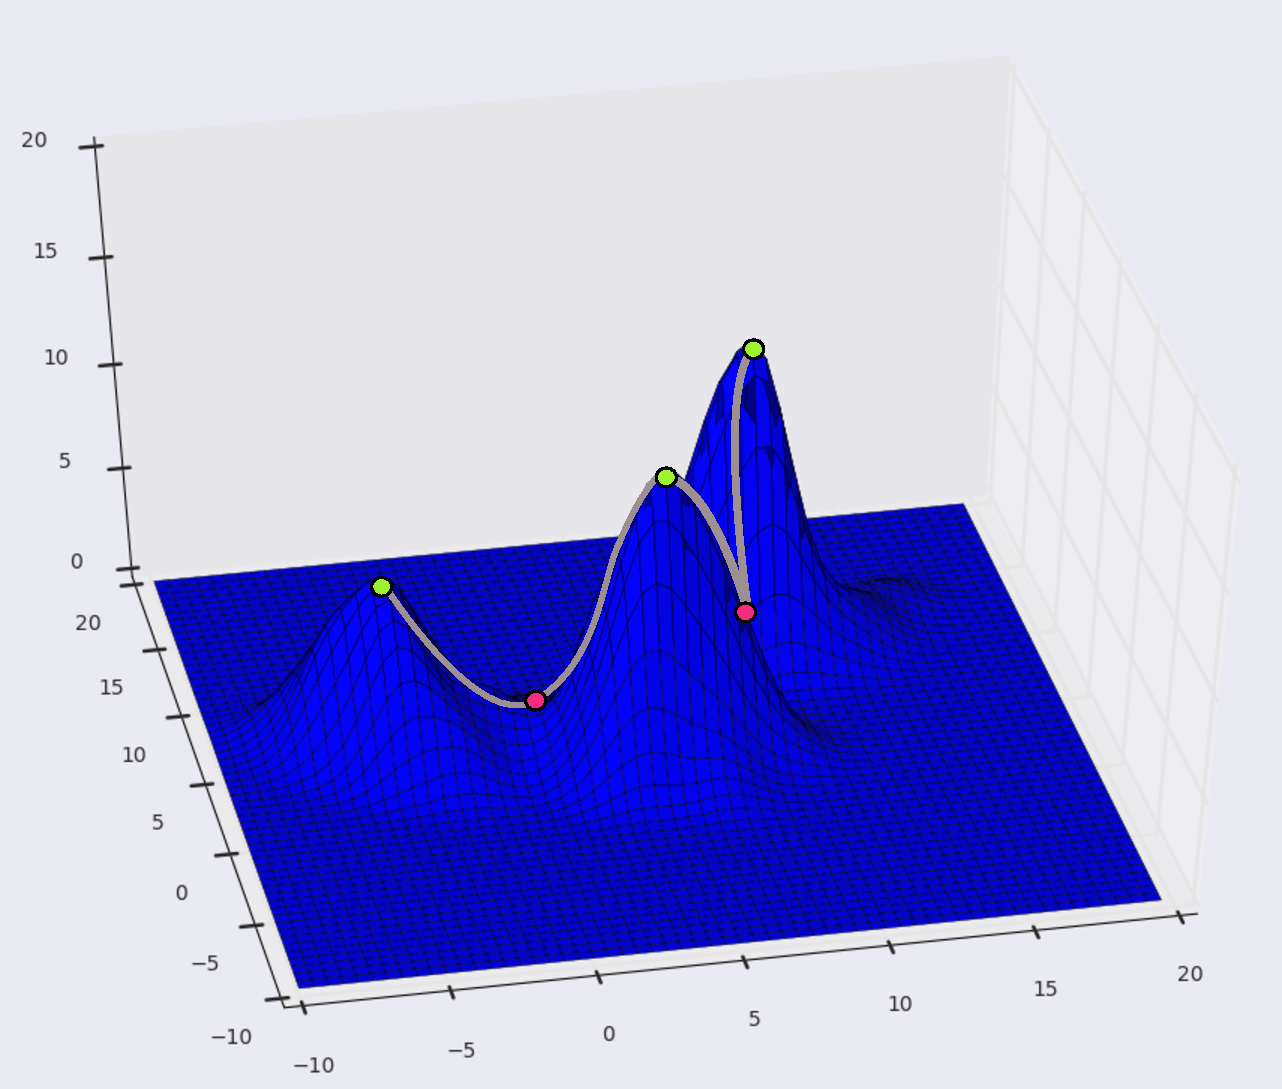
\includegraphics[scale=0.25]{ridges}
    \caption{KDE}
  \end{figure}

  \begin{block}{}
    If the samples are concentrated around a graph, then the mountain ridges on
    the graph of the density function are expected to capture it.
  \end{block}
\end{frame}

\begin{frame}{Conclusion}
  \begin{enumerate}
  \item our project is ongoing.
  \item there is a reading group in mathematics department meeting weekly to
    discuss Morse theory.
  \end{enumerate}
\end{frame}

\begin{frame}
  \centering
  \Huge{\textcolor{magenta}{Thanks}}
\end{frame}
\end{document}
